\subsubsection{Galvanic skin reaction and temperature data;}
\label{subsubsec:results_gsr_temp_2}

The GSR analysis is also made by analyzing its average and comparing both features between both blind and sample groups. As mentioned before, there was no influence of the temperature and the GSR sensor was worn on the left hand for right-handed participant and on the right hand for left-handed participants.

The Table \ref{tab:gsr_table_noBase} presents the average skin conductance by each participant on each scenes and they are plotted in the Figures \ref{fig:barplot_ecg_sdnn_4_scene_blind} to \ref{fig:barplot_ecg_sdnn_4_scene}.

The Table \ref{tab:gsr_var_noBase} presents the average skin conductance by each participant on their baseline and on each scene and their respectivily variation is inside Table \ref{tab:gsr_var_blind}. In the majority of times the skin conductance has risen from the "First" to the "Return" round, which mean that the participant was more aroused or with a higher mental workload.


\begin{table}[!htb]
\centering
\caption{Average GSR felled by the participants [$\mu$S].}
\label{tab:gsr_table_noBase}
\begin{tabular}{lllrrrrrr}
\toprule
    &       &        & Baseline &  Audio & \begin{tabular}[c]{@{}l@{}}Haptic\\ Belt\end{tabular} & \begin{tabular}[c]{@{}l@{}}Virtual\\ Cane\end{tabular} & Mixture \\
Participant & Visual Condition & Round &          &        &                                                       &                                                        &         \\
\midrule
001C & Blind & First &     0.37 &   1.03 &                                                  3.14 &                                                   3.79 &    3.90 \\
    &       & Return &          &   1.58 &                                                  2.81 &                                                   4.04 &    4.57 \\
003C & Blind & First &     0.30 &   0.56 &                                                  0.62 &                                                   0.85 &    1.09 \\
    &       & Return &          &   0.63 &                                                  0.65 &                                                   0.92 &    1.06 \\
004C & Blind & First &     1.24 &   3.07 &                                                  3.49 &                                                   2.28 &    2.23 \\
    &       & Return &          &   2.95 &                                                  3.20 &                                                   2.21 &    2.24 \\
001 & Sight & First &     4.27 &  15.19 &                                                 15.67 &                                                  15.19 &   14.15 \\
    &       & Return &          &  14.95 &                                                 15.09 &                                                  15.72 &   21.52 \\
004 & Sight & First &     2.60 &  11.18 &                                                 12.60 &                                                  12.92 &   10.34 \\
    &       & Return &          &  11.97 &                                                 12.25 &                                                  13.47 &   10.16 \\
005 & Sight & First &     0.47 &   1.58 &                                                  1.44 &                                                   1.37 &    1.33 \\
    &       & Return &          &   1.53 &                                                  1.47 &                                                   1.49 &    1.33 \\
\bottomrule
\end{tabular}
\end{table}




\begin{table}[!htb]
\centering
\caption{Average GSR variation in relation to the baseline in each round [$\mu$S].}
\label{tab:gsr_var_noBase}
\begin{tabular}{lllrrrrrr}
\toprule
    &       &        &     Audio & \begin{tabular}[c]{@{}l@{}}Haptic\\ Belt\end{tabular} & \begin{tabular}[c]{@{}l@{}}Virtual\\ Cane\end{tabular} &    Mixture \\
Participant & Visual Condition & Round &           &                                                       &                                                        &            \\
\midrule
001 & Sight & First &  255.76\% &                                              266.93\% &                                               255.69\% &   231.52\% \\
    &       & Return &  250.18\% &                                              253.32\% &                                               268.25\% &   403.90\% \\
001C & Blind & First &  176.54\% &                                              746.10\% &                                               920.72\% &   951.71\% \\
    &       & Return &  327.42\% &                                              656.99\% &                                               988.93\% &  1132.39\% \\
003C & Blind & First &   84.23\% &                                              104.19\% &                                               182.35\% &   258.80\% \\
    &       & Return &  109.23\% &                                              112.95\% &                                               202.35\% &   249.72\% \\
004 & Sight & First &  329.08\% &                                              383.54\% &                                               395.83\% &   297.05\% \\
    &       & Return &  359.53\% &                                              370.35\% &                                               417.17\% &   289.96\% \\
004C & Blind & First &  148.53\% &                                              182.84\% &                                                84.33\% &    80.69\% \\
    &       & Return &  138.64\% &                                              159.00\% &                                                78.73\% &    81.61\% \\
005 & Sight & First &  239.16\% &                                              207.74\% &                                               193.85\% &   184.71\% \\
    &       & Return &  227.06\% &                                              214.91\% &                                               219.59\% &   185.86\% \\
\bottomrule
\end{tabular}
\end{table}



The Figures \ref{fig:barplot_gsr_avg_4_scene_blind} show a pattern, that the presence of a haptic device increases the GSR variation, hence the stress or the mental workload, and \ref{fig:barplot_gsr_avg_4_scene_sight} do not show a pattern, all GSR variations are basic the same. One thing in common is that the "Haptic belt" caused a deacreased between the rounds, while the other methods caused an increase.

The Figure \ref{fig:barplot_gsr_avg_4_scene} reinforces the fact that the presence of a haptic device increases the GSR for the blind user. With those devices, the blind user's GSR were higher than the sighted user. The opposite happened in the "Audio" method.

\begin{figure}[!htb]
    \centering
    \begin{minipage}{\textwidth}
        \centering
        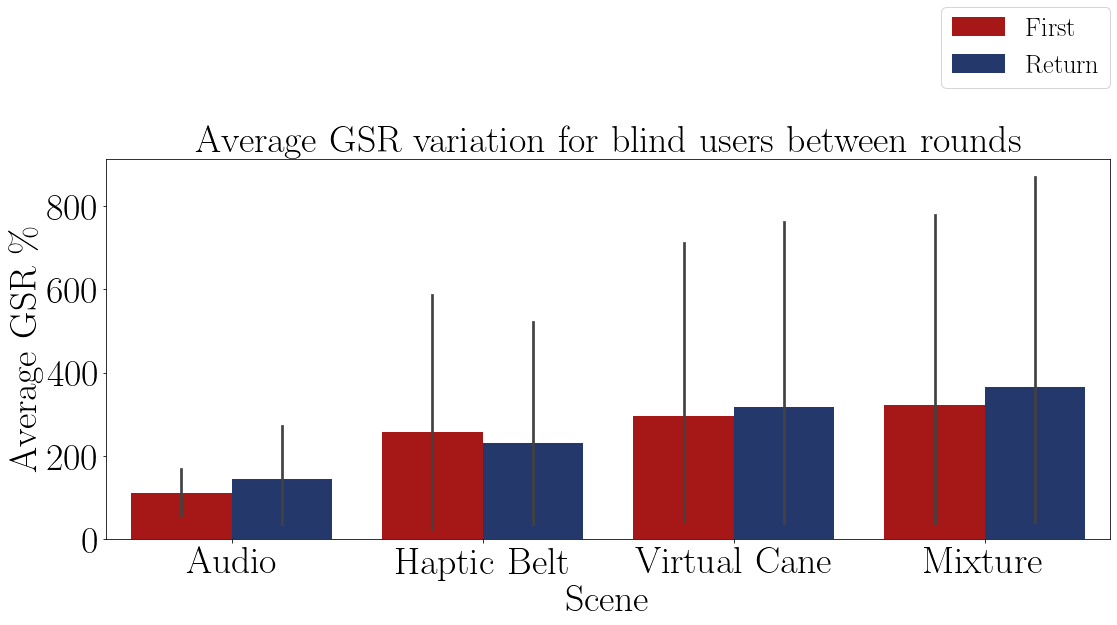
\includegraphics[width = 0.8\linewidth]{Resultados/GSR/Figuras/png/barplot_gsr_avg_4_scene_blind.png}
        \caption{Barplot of the average GSR of the blind participants on each method and round.}
        \label{fig:barplot_gsr_avg_4_scene_blind}
    \end{minipage}
    \begin{minipage}{\textwidth}
        \centering
        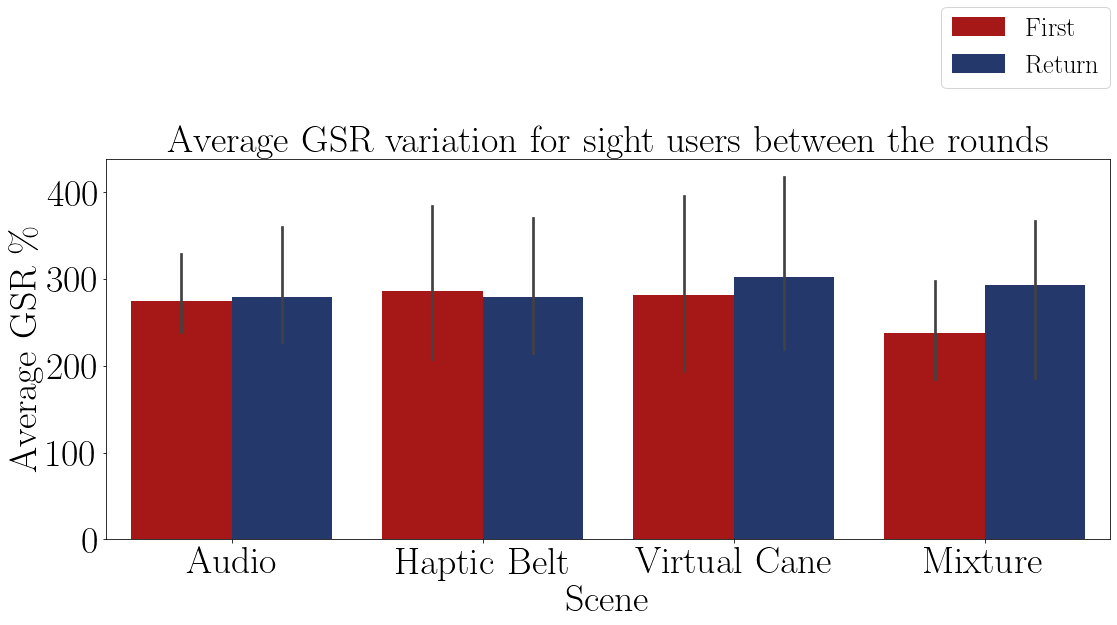
\includegraphics[width = 0.8\linewidth]{Resultados/GSR/Figuras/png/barplot_gsr_avg_4_scene_sight.png}
        \caption{Barplot of the average GSR of the sight participants on each method and round.}
        \label{fig:barplot_gsr_avg_4_scene_sight}
    \end{minipage}
\end{figure}
\begin{figure}[!htb]
    \centering
    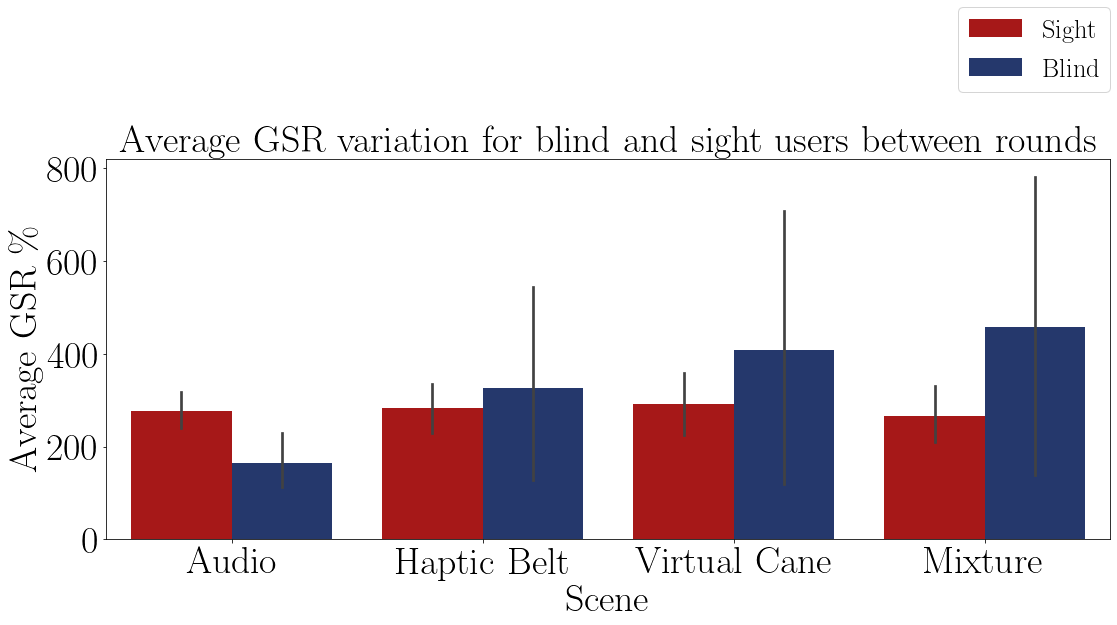
\includegraphics[width = 0.8\linewidth]{Resultados/GSR/Figuras/png/barplot_gsr_avg_4_scene.png}
    \caption{Barplot of the average GSR of both participants on each method.}
    \label{fig:barplot_gsr_avg_4_scene}
\end{figure}

The Figure \ref{fig:boxplot_ecg_sdnn_4_scene} and \ref{fig:boxplot_ecg_sdnn_4_rounds} presents a box plot with the average skin conductance of both groups by method and rounds in that order. These figures show the reaction of the sight user was different from the blind users. In all methods the GSR for the sighted user appears to be more constant. The effect of the round appear to be the same for both of the groups, none.

\begin{figure}[!htb]
    \centering
    \begin{minipage}{0.45\textwidth}
        \centering
        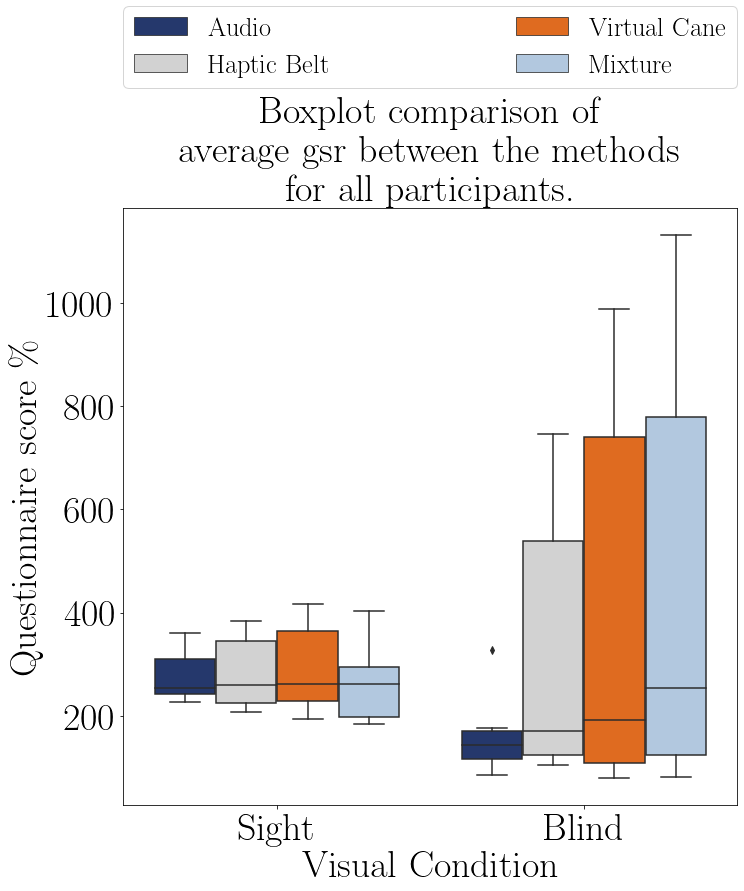
\includegraphics[width = 0.8\linewidth]{Resultados/GSR/Figuras/png/boxplot_gsr_avg_4_scene.png}
        \caption{Boxplot of the average GSR of the participants grouped by method.}
        \label{fig:boxplot_gsr_avg_4_scene}
    \end{minipage}
    \begin{minipage}{0.45\textwidth}
        \centering
        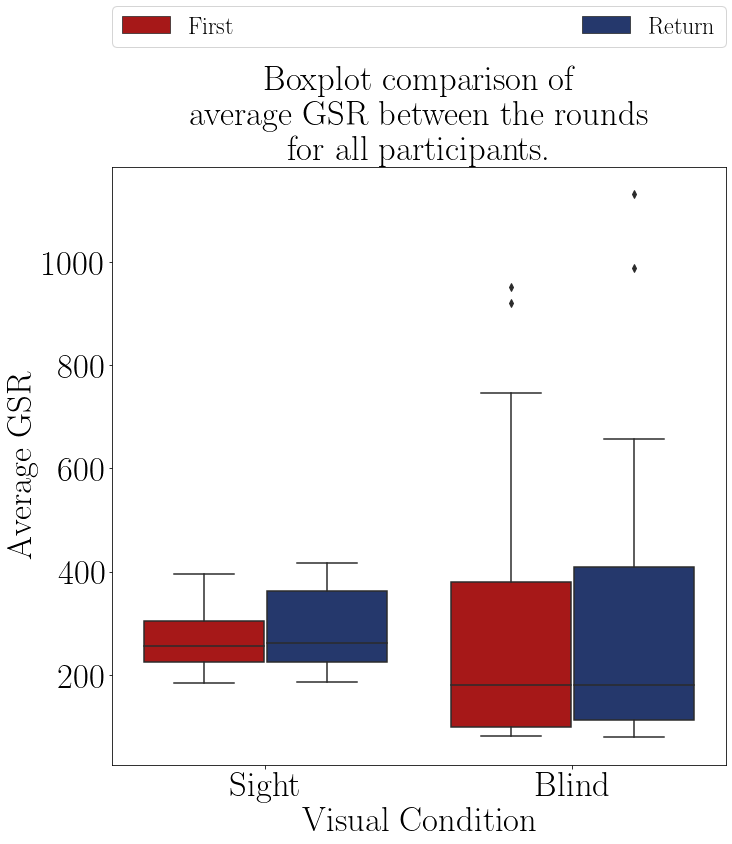
\includegraphics[width = 0.8\linewidth]{Resultados/GSR/Figuras/png/boxplot_gsr_avg_4_rounds.png}
        \caption{Boxplot of the average GSR of the participants grouped by round.}
        \label{fig:boxplot_gsr_avg_4_rounds}
    \end{minipage}
\end{figure}
 
The Table \ref{tab:gsr_average_group_noBase} shows the average skin conductance variation of both samples. It also shows that the presence of a haptic device increases the GSR, whilst the sight user had a basically constant GSR.


\begin{table}[!htb]
\centering
\caption{Average GSR variation grouped by participant and visual condition}
\label{tab:gsr_average_group_noBase}
\begin{tabular}{lrrrrr}
\toprule
{} &     Audio & \begin{tabular}[c]{@{}l@{}}Haptic\\ Belt\end{tabular} & \begin{tabular}[c]{@{}l@{}}Virtual\\ Cane\end{tabular} &   Mixture \\
Visual Condition &           &                                                       &                                                        &           \\
\midrule
Blind            &  164.10\% &                                              327.01\% &                                               409.57\% &  459.15\% \\
Sight            &  276.80\% &                                              282.80\% &                                               291.73\% &  265.50\% \\
\bottomrule
\end{tabular}
\end{table}



The Figures \ref{fig:qqplot_gsr_two_way_sight} and \ref{fig:residplot_gsr_two_way_sight} shows the distribution and variance of sighted participants of the Table \ref{tab:gsr_table_noBase}. These Figures shows that the data are normally distributed and that the methods have a similar variance.
The Table \ref{tab:blocanova_gsr_two_way_sight} shows the ANOVA test p-values of the average skin conductance variance of the "sight" sample between the guidance methods and they show that nor the methods nor the rounds had an effect on the sight users.


\begin{table}[!htb]
\centering
\caption{Anova p-value for the skin conductance average on each method for blinded users.}
\label{tab:blocanova_gsr_two_way_sight}
\begin{tabular}{lrrrrl}
\toprule
          Source & P-Value \\
\midrule
    \    Methods &   0.802 \\
     \    Rounds &   0.354 \\
\    Interaction &   0.686 \\
\bottomrule
\end{tabular}
\end{table}



\begin{figure}[!htb]
    \centering
    \begin{minipage}{0.45\textwidth}
        \centering
        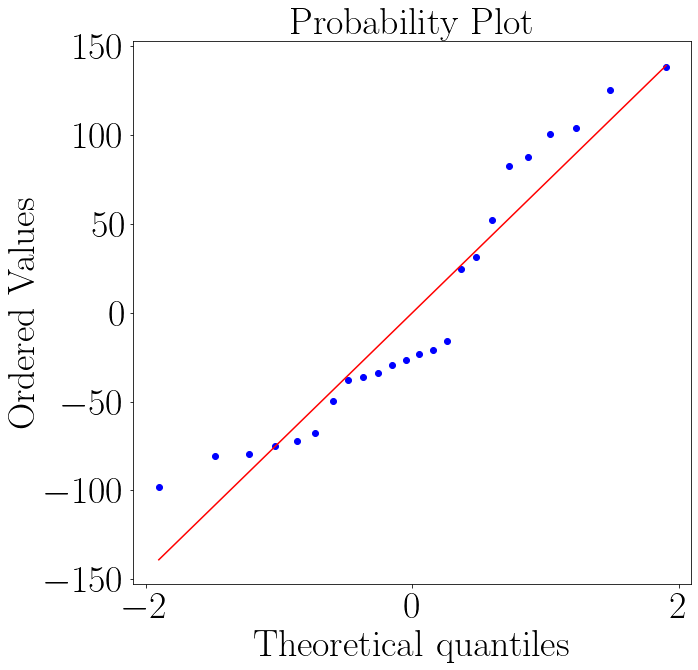
\includegraphics[width = 0.8\linewidth]{Resultados/GSR/Figuras/png/qqplot_gsr_two_way_sight.png}
        \caption{QQ plot of the average skin conductance of the sight participants on each method.}
        \label{fig:qqplot_gsr_two_way_sight}
    \end{minipage}
    \begin{minipage}{0.45\textwidth}
        \centering
        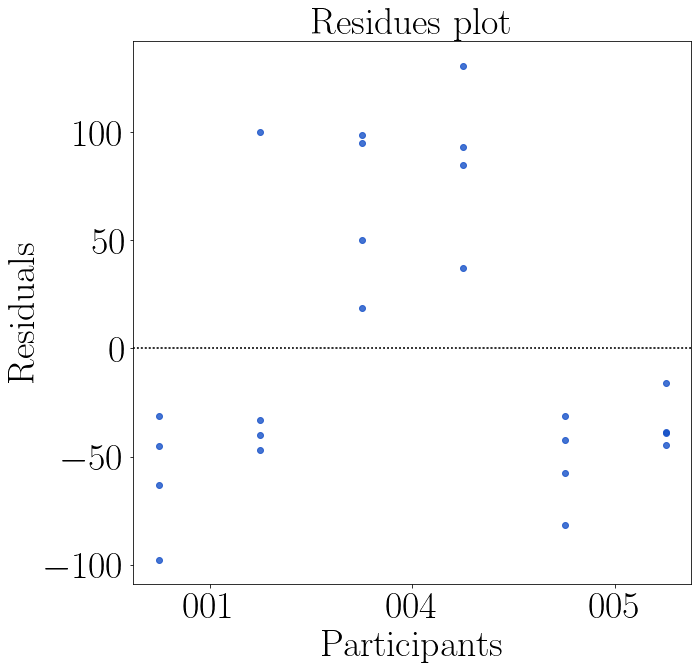
\includegraphics[width = 0.8\linewidth]{Resultados/GSR/Figuras/png/residplot_gsr_two_way_sight.png}
        \caption{Residual plot of the average skin conductance score the sight participants on each method.}
        \label{fig:residplot_gsr_two_way_sight}
    \end{minipage}
\end{figure}


%
\begin{table}[!htb]
\centering
\caption{Cross validation p-value for the skin conductance average on each method for blinded users.}
\label{tab:lsd_gsr_two_way_sight}
\begin{tabular}{rclr}
\toprule
      \multicolumn{3}{c}{Method} &                                       Analysis \\
\midrule
       Audio & $X$ & Haptic Belt &        $H_0 : \mu_{Audio} = \mu_{Haptic Belt}$ \\
      Audio & $X$ & Virtual Cane &   $H_1 : \mu_{Audio} \ne \mu_{Virtual Cane}**$ \\
           Audio & $X$ & Mixture &            $H_0 : \mu_{Audio} = \mu_{Mixture}$ \\
Haptic Belt & $X$ & Virtual Cane & $H_0 : \mu_{Haptic Belt} = \mu_{Virtual Cane}$ \\
     Haptic Belt & $X$ & Mixture &  $H_1 : \mu_{Haptic Belt} \ne \mu_{Mixture}**$ \\
    Virtual Cane & $X$ & Mixture & $H_1 : \mu_{Virtual Cane} \ne \mu_{Mixture}**$ \\
\bottomrule
\end{tabular}
\end{table}


%
%The Table \ref{tab:lsd_gsr_two_way_sight} presents the conclusion of a pairwise Fisher LSD test of the blind heart rate frequency variation between all the guidance methods and it shows that all methods had different effect on the heartrate, appart of the "Virtual Cane" and "Mixture", which presented similar SDNN.

According to the ANOVA test at Table \ref{tab:blocanova_gsr_two_way_sight} the methods did not impact the sight user's arousal or their mental workload. This was the same result from the ANOVA test of the Section \ref{subsubsec:results_gsr_temp_1}. The Figure \ref{fig:boxplot_gsr_avg_4_scene} showed the same result, but the same was not said about the boxplot of the blind user.

\FloatBarrier